\documentclass{VUMIFPSkursinis}
\usepackage{algorithmicx}
\usepackage{algorithm}
\usepackage{algpseudocode}
\usepackage{amsfonts}
\usepackage{amsmath}
\usepackage{bm}
\usepackage{caption}
\usepackage{color}
\usepackage{float}
\usepackage{graphicx}
\usepackage{listings}
\usepackage{subfig}
\usepackage{wrapfig}
\usepackage{sectsty}
\usepackage{enumerate}
\usepackage{longtable}
\usepackage[export]{adjustbox}
\usepackage{rotating}
\usepackage{hhline}
\usepackage{multirow}
\usepackage{tabularx}
\usepackage{array}
\usepackage{booktabs,calc}
\usepackage{tabularx,colortbl}
\usepackage[table]{xcolor}  
\usepackage{longtable}  

\usepackage{enumitem}
%PAKEISTA, tarpai tarp sąrašo elementų
\setitemize{noitemsep,topsep=0pt,parsep=0pt,partopsep=0pt}
\setenumerate{noitemsep,topsep=0pt,parsep=0pt,partopsep=0pt}
\allsectionsfont{\centering}
% Titulinio aprašas
\university{Vilniaus universitetas}
\faculty{Matematikos ir informatikos fakultetas}
\department{Programų sistemų katedra}
\papertype{Programų sistemų inžinerijos II laboratorinis darbas}
\title{Socialinis Vilniaus universiteto tinklalapis}
\titleineng{SocialVU}
\status{2 kurso 4 grupės studentai}
\author{Andrejus Voitovas}
\secondauthor{Eglė Puodžiūnaitė}
\thirdauthor{Kasparas Kralikas}
\fourthauthor{Ieva Vizgirdaitė} % Pridėti antrą autorių
\supervisor{asist. dr. Vytautas Valaitis}
\date{Vilnius – \the\year}

% Nustatymai
% \setmainfont{Palemonas}   % Pakeisti teksto šriftą į Palemonas (turi būti įdiegtas sistemoje)
\bibliography{bibliografija}

\begin{document}
% PAKEISTA
\maketitle
\cleardoublepage\pagenumbering{arabic}
\setcounter{page}{2}
\sectionnonum{ANOTACIJA}
Šiame dokumente specifikuojami kuriamos sistemos reikalavimai. Jie nagrinėjami trimis etapais. Pirmiausia aprašomi funkciniai reikalavimai, detaliai apibrėžiantys pagrindines ir pagalbines sistemos funkcijas. Toliau nagrinėjami nefunkciniai reikalavimai, apibrėžiantys kaip sistema turi veikti ir kaip ji turi būti kuriama. Galiausiai nusakomi vartotojo sąsąjos reikalavimai, kur pateikiami metaforos reikalavimai, formuluojamos užduotys, užduočių formulavimo kalbos reilkalavimai, užduočių formulavimo protokolo reikalavimai, interfeiso darnos ir standartizavimo reikalavimai, pranešimų formulavimo reikalavimai ir interfeiso individualizavimo reikalavimai.
\\Rašant šį dokumentą buvo naudojamasi:
\\1. dr. Vytauto Valaičio Internetinis puslapiu (https://klevas.mif.vu.lt/~valaitis/)
\\2. doc., dr. Karolio Petrausko internetiniu puslapiu (http://klevas.mif.vu.lt/~karolis/)
\\3. Latex programa
\\4. lab. asst. Jono Brusoko parengtais kursinio darbo šablonais (https://gitlab.com/JohnLogic/SE-course-work-template)
\newpage
%TURINYS
\tableofcontents
\sectionnonum{ĮVADAS}
Šio dokumento tikslas - pateikti tikslius reikalavimus kuriamam socialiniam tinklapiui, kuris palengvintų universiteto bendruomenės tarpusavio komunikaciją.
\\\textbf{Temos aktualumas}
\\Šiuo metu studentams dėstytojų skelbiama informacija yra išbarstyta internete, kurią norint surasti, prireikia nemažai laiko ir pastangų. Internete egzistuoja atskiras universiteto naujienų puslapis, o kiekvienas dėstytojas turi savo asmeninį tinklalapį bei atskirą elektroninį paštą. Tiek dėstytojui pasiekti studentus, tiek studentui - dėstytoją yra komplikuota ir labai nepatogu.
\\\textbf{Dalykinė sritis}
\\Socialinis Vilniaus Universiteto tinklapis.
\\\textbf{Probleminė sritis} 
\\Socialinis Vilniaus Universiteto tinklapis suteiktų galimybę greitai ir paprastai pasiekti šio universiteto dėstytotjų puslapius, leistų susisiekti su pačiais dėstytojais. Pagrindinis tinklapio išskirtinumas - greitai ir patogiai pasiekiama informacija - viskas vienoje vietoje.
\\\textbf{Darbo pagrindas}
\\Dokumentas parengtas kaip Programų sistemų inžinerijos II laboratorinis darbas.
\\\textbf{Darbo užduotys}
\\1. Suformuluoti funkcinius reikalavimus
\\2. Suformuluoti nefunkcinius reikalavimus
\\3. Suformuluoti vartotojo sąsąjos reikalavimus
\\4. Atsižvelgiant į šio darbo turinį, atitinkamai pakoreguoti programų sistemų inžinerijos I laboratorinį darbą 


\newpage

\section{FUNKCINIAI REIKALAVIMAI}
Šiame skyriuje pateikiami funkciniai reikalavimai – nagrinėjami scenarijai, ką sistema turi daryti, kaip elgtis vienu ar kitu atveju. Apibrėžiant funkcinius reikalavimus naudojamos procesų sekų diagramos, sistemoje vykdomų užduočių diagramos.
\subsection{Internetinės svetainės langai}
	\begin{table}[H]
	\caption{Funkciniai reikalavimai. Internetinės svetainės langai.}
	\begin{tabular}{|p{1cm}|p{1cm}|p{11,5cm}|p{3,5cm}|}
		\hline 
		\rowcolor{gray!50}
		\multicolumn{2}{|c|}{{\bfseries Kodas}}&
		\multicolumn{1}{c|}{{\bfseries Reikalavimas}}&
		\multicolumn{1}{c|}{{\bfseries Svarba}}\\
		\hline
		\rowcolor{lightgray}
		\multicolumn{4}{|c|}{Internetinės svetainės langai}\\		
		
		\hline
		\multicolumn{2}{|c|}{FR 1.1}&
		{Svetainės langas „Prisijungimas“ turi būti matomas visiems net ir neprisijungusiems naudotojams.
		}&		
		\multicolumn{1}{c|}{Būtina}\\
		\hline
		\multicolumn{1}{|c}{}&
		\multicolumn{1}{c|}{FR 1.2}&
		{Svetainės langai „Pagrindinis puslapis“, „Dėstytojai“, „Dėstytojo puslapis“, „D.U.K.“, „Renginiai“, „Žinutės“, „Mano profilis“, „Renginio informacija“ turi būti matomi visiems prisijungusiems naudotojams.
		}&		
		\multicolumn{1}{c|}{Būtina}\\
		\hline
		\multicolumn{1}{|c}{}&
		\multicolumn{1}{c|}{FR 1.3}&
		{Svetainės langas „Konspektai“ turi būti matomas visiems prisijungusiems studentams bei sistemos adminstratoriams.
		}&
		\multicolumn{1}{c|}{Būtina}\\	
		\hline		
		\multicolumn{1}{|c}{}&
		\multicolumn{1}{c|}{FR 1.4}&
		{Svetainės langas „Dėstytojo puslapio redagavimas“ turi būti matomas visiems prisijungusiam puslapį sukūrusiam dėstytojui.
		}&
		\multicolumn{1}{c|}{Būtina}\\									
		\hline
	\end{tabular}		
\end{table}

\subsection{Prisijungimas}
	\begin{table}[H]
	\caption{Funkciniai reikalavimai. Prisijungimas.}
	\begin{tabular}{|p{1cm}|p{1cm}|p{11,5cm}|p{3,5cm}|}
		\hline 
		\rowcolor{gray!50}
		\multicolumn{2}{|c|}{{\bfseries Kodas}}&
		\multicolumn{1}{c|}{{\bfseries Reikalavimas}}&
		\multicolumn{1}{c|}{{\bfseries Svarba}}\\
		\hline
		\rowcolor{lightgray}
		\multicolumn{4}{|c|}{Prisijungimas}\\		
		
		\hline
		\multicolumn{2}{|c|}{FR 2.1}&
		{Naudotojui suvedus tinkamus prisijungimo duomenis jis turi būti prijungiamas prie sistemos.
		}&		
		\multicolumn{1}{c|}{Būtina}\\
		\hline
		\multicolumn{1}{|c}{}&
		\multicolumn{1}{c|}{FR 2.2}&
		{Naudotojui netinkamai įvedus prisijungimo duomenis jis neturi būti prijungiamas prie sistemos ir turi būti išmetamas klaidos pranešimas.
		}&		
		\multicolumn{1}{c|}{Būtina}\\
		\hline
		\multicolumn{1}{|c}{}&
		\multicolumn{1}{c|}{FR 2.3}&
		{Turi būti galimybė užmiršus slaptažodį gautį naują slaptažodį į el. paštą.
		}&
		\multicolumn{1}{c|}{Pageidaujama}\\	
		\hline		
		\multicolumn{1}{|c}{}&
		\multicolumn{1}{c|}{FR 2.4}&
		{Naudotojų bandymų prisijungti prie sistemos skaičius neturi būti ribojamas.
		}&
		\multicolumn{1}{c|}{Būtina}\\									
		\hline
	\end{tabular}		
\end{table}
\ref{fig:login} pav. pateikiama užduoties „Prisijungimas” sekų diagrama. Joje vaizduojamas pagrindinis prisijungimo prie sistemos scenarijus ir taip pat nagrinėjami alternatyvūs scenarijai.
\begin{figure}[H]
	\centering
	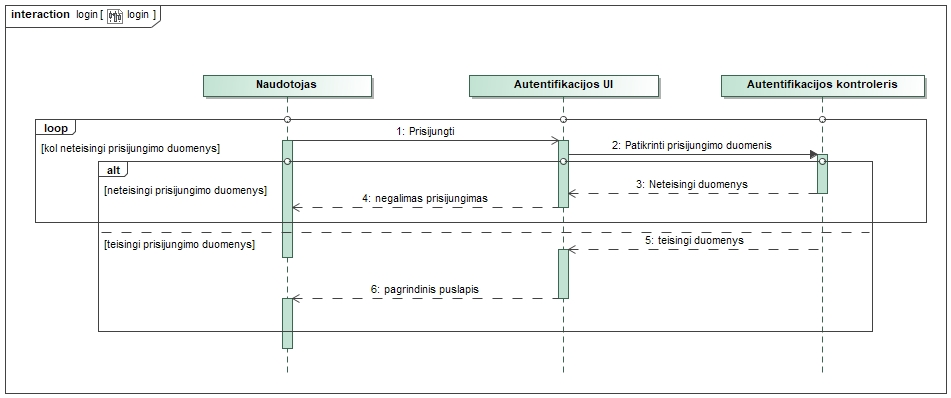
\includegraphics[width=\linewidth]{img/login.jpg}
	\caption{Proceso „Prisijungimas“ sekų diagrama}
	\label{fig:login}
\end{figure}

\subsection{Atsijungimas}

	\begin{table}[H]
	\caption{Funkciniai reikalavimai. Atsijungimas.}
	\begin{tabular}{|p{1cm}|p{1cm}|p{11,5cm}|p{3,5cm}|}
		\hline 
		\rowcolor{gray!50}
		\multicolumn{2}{|c|}{{\bfseries Kodas}}&
		\multicolumn{1}{c|}{{\bfseries Reikalavimas}}&
		\multicolumn{1}{c|}{{\bfseries Svarba}}\\
		\hline
		\rowcolor{lightgray}
		\multicolumn{4}{|c|}{Atsijungimas}\\		
		
		\hline
		\multicolumn{2}{|c|}{FR 3.1}&
		{Naudotojas paspaudęs mygtuką atsijungti turi būti atjungiamas nuo sistemos.
		}&		
		\multicolumn{1}{c|}{Būtina}\\
		\hline
		\multicolumn{1}{|c}{}&
		\multicolumn{1}{c|}{FR 3.2}&
		{Atsijungus nuo sistemos ir bandant paspausti grįžimo mygtuką naudotojas turi būti nukreipiamas į prisijungimo langą.
		}&		
		\multicolumn{1}{c|}{Būtina}\\
		\hline
	\end{tabular}		
\end{table}

\subsection{Paskyros valdymas}

	\begin{table}[H]
	\caption{Funkciniai reikalavimai. Paskyros valdymas.}
	\begin{tabular}{|p{1cm}|p{1cm}|p{11,5cm}|p{3,5cm}|}
		\hline 
		\rowcolor{gray!50}
		\multicolumn{2}{|c|}{{\bfseries Kodas}}&
		\multicolumn{1}{c|}{{\bfseries Reikalavimas}}&
		\multicolumn{1}{c|}{{\bfseries Svarba}}\\
		\hline
		\rowcolor{lightgray}
		\multicolumn{4}{|c|}{Paskyros valdymas}\\				
		\hline
		\multicolumn{2}{|c|}{FR 4.1}&
		{Naudotojui paspaudus mygtuką „Mano profilis“ turi būti matoma visa žinoma informacija apie naudotoją.
		}&		
		\multicolumn{1}{c|}{Būtina}\\
		\hline
		\multicolumn{1}{|c}{}&
		\multicolumn{1}{c|}{FR 4.2}&
		{Naudotojui paspaudus mygtuką „Pakeisti slaptažodį“, įvedus tinkamą seną ir naują slaptažodžius bei paspaudus mygtuką „Patvirtinti“ slaptažodis turi būti pakeičiamas į naują.
		}&		
		\multicolumn{1}{c|}{Būtina}\\
		\hline
		\multicolumn{1}{|c}{}&
		\multicolumn{1}{c|}{FR 4.3}&
		{Naudotojui paspaudus mygtuką „Pakeisti slaptažodį“ ir įvedus netinkamą seną slaptažodį turi būti išvedamas klaidos pranešimas.
		}&
		\multicolumn{1}{c|}{Būtina}\\	
		\hline		
		\multicolumn{1}{|c}{}&
		\multicolumn{1}{c|}{FR 4.4}&
		{Naudotojui paspaudus mygtuką „Pakeisti slaptažodį“ ir įvedus netinkamo formato naują slaptažodį turi būti išvedamas klaidos pranešimas ir slaptažodis neturi būti pakeičiamas nauju.
		}&
		\multicolumn{1}{c|}{Būtina}\\									
		\hline
	\end{tabular}		
\end{table}

\subsection{Naujienos}

\begin{table}[H]
	\caption{Funkciniai reikalavimai. Naujienos.}
	\begin{tabular}{|p{1cm}|p{1cm}|p{11,5cm}|p{3,5cm}|}
		\hline 
		\rowcolor{gray!50}
		\multicolumn{2}{|c|}{{\bfseries Kodas}}&
		\multicolumn{1}{c|}{{\bfseries Reikalavimas}}&
		\multicolumn{1}{c|}{{\bfseries Svarba}}\\
		\hline
		\rowcolor{lightgray}
		\multicolumn{4}{|c|}{Naujienos}\\		
		
		\hline
		\multicolumn{2}{|c|}{FR 5.1}&
		{Naujienos turi būti matomos pagrindiniame tinklalapio puslapyje.
		}&		
		\multicolumn{1}{c|}{Būtina}\\
		\hline
		\multicolumn{1}{|c}{}&
		\multicolumn{1}{c|}{FR 5.2}&
		{Visas naujienų sąrašas turi būti pateikiamas viename puslapyje.
		}&		
		\multicolumn{1}{c|}{Būtina}\\
		\hline
		\multicolumn{1}{|c}{}&
		\multicolumn{1}{c|}{FR 5.3}&
		{Naujienos turi būti rikiuojamos pagal naujienos paskelbimo datą (naujausios turi būti matomos pirmos).
		}&
		\multicolumn{1}{c|}{Būtina}\\	
		\hline		
		\multicolumn{1}{|c}{}&
		\multicolumn{1}{c|}{FR 5.4}&
		{Jei naujienų sąrašas tuščias turi būti rodomas pranešimas, kad naujienų šiuo metu nėra.
		}&
		\multicolumn{1}{c|}{Būtina}\\									
		\hline
		\multicolumn{1}{|c}{}&
		\multicolumn{1}{c|}{FR 5.5}&
		{Naujienos turi būti matomos visiems prisijungusiems naudotojams.
		}&
		\multicolumn{1}{c|}{Būtina}\\	
		\hline		
		\multicolumn{1}{|c}{}&
		\multicolumn{1}{c|}{FR 5.6}&
		{Naujienos redagavimo funkcija turi būti matoma bei panaudojama tik naujieną paskelbusiam naudotojui.
		}&
		\multicolumn{1}{c|}{Būtina}\\									
		\hline
		\multicolumn{1}{|c}{}&
		\multicolumn{1}{c|}{FR 5.7}&
		{Skelbti naujienas turi būti galimybė tik prisijungusiems dėstytojams bei sistemos administratoriams.
		}&
		\multicolumn{1}{c|}{Būtina}\\	
		\hline		
		\multicolumn{1}{|c}{}&
		\multicolumn{1}{c|}{FR 5.8}&
		{Naujienos ištrynimo funkcija turi būti matoma bei panaudojama tik naujieną paskelbusiam naudotojui bei sistemos administratoriui.
		}&
		\multicolumn{1}{c|}{Būtina}\\									
		\hline
	\end{tabular}		
\end{table}

\ref{fig:delnews} pav. pateikiama užduoties „Naujienos ištrynimas” sekų diagrama. Joje vaizduojamas pagrindinis
naujienos ištrynimo scenarijus.
\begin{figure}[H]
	\centering
	\includegraphics[width=\linewidth]{img/deleteNew.png}
	\caption{Proceso „Naujienos ištrynimas“ sekų diagrama}
	\label{fig:delnews}
\end{figure}

\subsection{Renginiai}

\begin{table}[H]
	\caption{Funkciniai reikalavimai. Renginiai.}
	\begin{tabular}{|p{1cm}|p{1cm}|p{11,5cm}|p{3,5cm}|}
		\hline 
		\rowcolor{gray!50}
		\multicolumn{2}{|c|}{{\bfseries Kodas}}&
		\multicolumn{1}{c|}{{\bfseries Reikalavimas}}&
		\multicolumn{1}{c|}{{\bfseries Svarba}}\\
		\hline
		\rowcolor{lightgray}
		\multicolumn{4}{|c|}{Renginiai}\\		
		
		\hline
		\multicolumn{2}{|c|}{FR 6.1}&
		{Renginiai turi būti matomi puslapyje „Renginiai“.
		}&		
		\multicolumn{1}{c|}{Būtina}\\
		\hline
		\multicolumn{1}{|c}{}&
		\multicolumn{1}{c|}{FR 6.2}&
		{Visas renginių sąrašas turi būti pateikiamas kalendoriuje esančiame puslapyje „Renginiai“.
		}&		
		\multicolumn{1}{c|}{Būtina}\\
		\hline
		\multicolumn{1}{|c}{}&
		\multicolumn{1}{c|}{FR 6.3}&
		{Paspaudus ant kalendoriuje pateikto renginio turi atsidaryti puslapis „Renginio informacija“, kuriame renginys turi būti aprašytas detaliau.
		}&
		\multicolumn{1}{c|}{Būtina}\\	
		\hline		
		\multicolumn{1}{|c}{}&
		\multicolumn{1}{c|}{FR 6.4}&
		{Jei nėra sukurta jokių renginiu, puslapyje „Renginiai“ turi būti pateikiamas tuščias kaledorius.
		}&
		\multicolumn{1}{c|}{Būtina}\\									
		\hline
		\multicolumn{1}{|c}{}&
		\multicolumn{1}{c|}{FR 6.5}&
		{Renginiai turi būti matomi visiems prisijungusiems naudotojams.
		}&
		\multicolumn{1}{c|}{Būtina}\\	
		\hline		
		\multicolumn{1}{|c}{}&
		\multicolumn{1}{c|}{FR 6.6}&
		{Renginio redagavimo funkcija turi būti matoma bei panaudojama tik renginį sukūrusiam naudotojui.
		}&
		\multicolumn{1}{c|}{Būtina}\\									
		\hline
		\multicolumn{1}{|c}{}&
		\multicolumn{1}{c|}{FR 6.7}&
		{Kurti renginius turi būti galimybė tik prisijungusiems dėstytojams bei sistemos administratoriams.
		}&
		\multicolumn{1}{c|}{Būtina}\\	
		\hline		
		\multicolumn{1}{|c}{}&
		\multicolumn{1}{c|}{FR 6.8}&
		{Renginio ištrynimo funkcija turi būti matoma bei panaudojama tik naujieną paskelbusiam naudotojui bei sistemos administratoriui.
		}&
		\multicolumn{1}{c|}{Būtina}\\									
		\hline
	\end{tabular}		
\end{table}

\ref{fig:addevent} pav. pateikiama užduoties „Renginio sukūrimas” sekų diagrama. Joje vaizduojamas pagrindinis
renginio sukūrimo scenarijus.
\begin{figure}[H]
	\centering
	\includegraphics[width=\linewidth]{img/addNewEvent.png}
	\caption{Proceso „Renginio sukūrimas“ sekų diagrama}
	\label{fig:addevent}
\end{figure}

\subsection{D.U.K.}
	\begin{table}[H]
	\caption{Funkciniai reikalavimai. D.U.K.}
	\begin{tabular}{|p{1cm}|p{1cm}|p{11,5cm}|p{3,5cm}|}
		\hline 
		\rowcolor{gray!50}
		\multicolumn{2}{|c|}{{\bfseries Kodas}}&
		\multicolumn{1}{c|}{{\bfseries Reikalavimas}}&
		\multicolumn{1}{c|}{{\bfseries Svarba}}\\
		\hline
		\rowcolor{lightgray}
		\multicolumn{4}{|c|}{D.U.K.}\\		
		
		\hline
		\multicolumn{2}{|c|}{FR 7.1}&
		{Dažniausiai užduodami klausimai turi būti matomi puslapyje „D.U.K.“.
		}&		
		\multicolumn{1}{c|}{Būtina}\\
		\hline
		\multicolumn{1}{|c}{}&
		\multicolumn{1}{c|}{FR 7.2}&
		{Visas dažniausiai užduodamų klausimų sąrašas turi būti pateikiamas viename puslapyje.
		}&		
		\multicolumn{1}{c|}{Būtina}\\
		\hline
		\multicolumn{1}{|c}{}&
		\multicolumn{1}{c|}{FR 7.3}&
		{Paspaudus ant vieno iš pateiktų klausimų turi būti matomas atsakymas į tą klausimą.
		}&
		\multicolumn{1}{c|}{Būtina}\\	
		\hline		
		\multicolumn{1}{|c}{}&
		\multicolumn{1}{c|}{FR 7.4}&
		{D.U.K. turi būti matomi visiems prisijungusiems naudotojams.
		}&
		\multicolumn{1}{c|}{Būtina}\\									
		\hline
		\multicolumn{1}{|c}{}&
		\multicolumn{1}{c|}{FR 7.5}&
		{D.U.K. redagavimo funkcija turi būti matoma bei panaudojama tik sistemos administratoriams.
		}&
		\multicolumn{1}{c|}{Būtina}\\	
		\hline	
		\multicolumn{1}{|c}{}&
		\multicolumn{1}{c|}{FR 7.6}&
		{Sukurti naują klausimą turi būti galimybė tik sistemos administratoriams.
		}&
		\multicolumn{1}{c|}{Būtina}\\	
		\hline	
		\multicolumn{1}{|c}{}&
		\multicolumn{1}{c|}{FR 7.7}&
		{Klausimo ištrynimo funkcija turi būti matoma bei panaudojama tik sistemos administratoriui.
		}&
		\multicolumn{1}{c|}{Būtina}\\	
		\hline	
	\end{tabular}		
\end{table}

\ref{fig:addduk} pav. pateikiama užduoties „D.U.K.pridėjimas” sekų diagrama. Joje vaizduojamas pagrindinis
D.U.K. pridėjimo scenarijus.
\begin{figure}[H]
	\centering
	\includegraphics[width=\linewidth]{img/addDUK.png}
	\caption{Proceso „D.U.K.pridėjimas” sekų diagrama}
	\label{fig:addduk}
\end{figure}

\subsection{Dėstytojų sąrašas}

	\begin{table}[H]
	\caption{Funkciniai reikalavimai. Dėstytojų sąrašas}
	\begin{tabular}{|p{1cm}|p{1cm}|p{11,5cm}|p{3,5cm}|}
		\hline 
		\rowcolor{gray!50}
		\multicolumn{2}{|c|}{{\bfseries Kodas}}&
		\multicolumn{1}{c|}{{\bfseries Reikalavimas}}&
		\multicolumn{1}{c|}{{\bfseries Svarba}}\\
		\hline
		\rowcolor{lightgray}
		\multicolumn{4}{|c|}{Dėstytojų sąrašas}\\		
		
		\hline
		\multicolumn{2}{|c|}{FR 8.1}&
		{Dėstytojų sąrašas turi būti matomas puslapyje „Dėstytojai“.
		}&		
		\multicolumn{1}{c|}{Būtina}\\
		\hline
		\multicolumn{1}{|c}{}&
		\multicolumn{1}{c|}{FR 8.2}&
		{Puslapyje „Dėstytojai“ turi būti paieškos laukas, kurio pagalba galima surasti reikiamą dėstytoją.
		}&		
		\multicolumn{1}{c|}{Būtina}\\
		\hline
		\multicolumn{1}{|c}{}&
		\multicolumn{1}{c|}{FR 8.3}&
		{Visas dėstytojų sąrašas turi būti pateikiamas viename puslapyje.
		}&
		\multicolumn{1}{c|}{Būtina}\\	
		\hline		
		\multicolumn{1}{|c}{}&
		\multicolumn{1}{c|}{FR 8.4}&
		{Dėstytojai turi būti surikiuoti abecėlės tvarka pagal pavardę ir vardą.
		}&
		\multicolumn{1}{c|}{Būtina}\\									
		\hline
		\multicolumn{1}{|c}{}&
		\multicolumn{1}{c|}{FR 8.5}&
		{Dėstytojų sąrašas turi būti matomas visiems prisijungusiems naudotojams.
		}&
		\multicolumn{1}{c|}{Būtina}\\	
		\hline	
		\multicolumn{1}{|c}{}&
		\multicolumn{1}{c|}{FR 8.6}&
		{Prie dėstytojo vardo bei pavardės turi būti pateikiamos nuorodos į dėstytojo puslapį bei į žinutės išsiuntimo dėstytojui puslapį.
		}&
		\multicolumn{1}{c|}{Būtina}\\	
		\hline		
	\end{tabular}		
\end{table}

\subsection{Dėstytojo puslapis}

	\begin{table}[H]
	\caption{Funkciniai reikalavimai. Dėstytojo puslapis}
	\begin{tabular}{|p{1cm}|p{1cm}|p{11,5cm}|p{3,5cm}|}
		\hline 
		\rowcolor{gray!50}
		\multicolumn{2}{|c|}{{\bfseries Kodas}}&
		\multicolumn{1}{c|}{{\bfseries Reikalavimas}}&
		\multicolumn{1}{c|}{{\bfseries Svarba}}\\
		\hline
		\rowcolor{lightgray}
		\multicolumn{4}{|c|}{Dėstytojo puslapis}\\		
		
		\hline
		\multicolumn{2}{|c|}{FR 9.1}&
		{Dėstytojo puslapis turi būti matomas visiems prisijungusiems naudotojams.
		}&		
		\multicolumn{1}{c|}{Būtina}\\
		\hline
		\multicolumn{1}{|c}{}&
		\multicolumn{1}{c|}{FR 9.2}&
		{Tik prisijungęs dėstytojas turi galimybę sukurti savo puslapį.
		}&		
		\multicolumn{1}{c|}{Būtina}\\
		\hline
		\multicolumn{1}{|c}{}&
		\multicolumn{1}{c|}{FR 9.3}&
		{Tik prisijungęs dėstytojas sukūręs savo puslapį turi galimybę jį redaguoti.
		}&
		\multicolumn{1}{c|}{Būtina}\\	
		\hline		
		\multicolumn{1}{|c}{}&
		\multicolumn{1}{c|}{FR 9.4}&
		{Dėstytojo puslapyje turi buti nuoroda, kurią paspaudus turi būti galimybė rašyti žinutę pasirinktam dėstytojui.
		}&
		\multicolumn{1}{c|}{Būtina}\\									
		\hline
	\end{tabular}		
\end{table}

\ref{fig:editpage} pav. pateikiama užduoties „Dėstytojo puslapio redagavimas” sekų diagrama. Joje vaizduojamas pagrindinis dėstytojo puslapio redagavimo scenarijus.
\begin{figure}[H]
	\centering
	\includegraphics[width=\linewidth]{img/editPage.png}
	\caption{Proceso „Dėstytojo puslapio redagavimas” sekų diagrama}
	\label{fig:editpage}
\end{figure}

\subsection{Žinutės}

	\begin{table}[H]
	\caption{Funkciniai reikalavimai. Žinutės}
	\begin{tabular}{|p{1cm}|p{1cm}|p{11,5cm}|p{3,5cm}|}
		\hline 
		\rowcolor{gray!50}
		\multicolumn{2}{|c|}{{\bfseries Kodas}}&
		\multicolumn{1}{c|}{{\bfseries Reikalavimas}}&
		\multicolumn{1}{c|}{{\bfseries Svarba}}\\
		\hline
		\rowcolor{lightgray}
		\multicolumn{4}{|c|}{Žinutės}\\		
		
		\hline
		\multicolumn{2}{|c|}{FR 10.1}&
		{Puslapis „Žinutės“ turi būti matomas visiems prisijungusiems naudotojams.
		}&		
		\multicolumn{1}{c|}{Būtina}\\
		\hline
		\multicolumn{1}{|c}{}&
		\multicolumn{1}{c|}{FR 10.2}&
		{Puslapyje „Žinutės“ turi būti pateikiamos visos gautos bei išsiųstos žinutės.
		}&		
		\multicolumn{1}{c|}{Būtina}\\
		\hline
		\multicolumn{1}{|c}{}&
		\multicolumn{1}{c|}{FR 10.3}&
		{Visoms gautoms bei išsiųstoms žinutėms pateikti naudojami puslapiai (viename puslapyje 25 žinutės).
		}&
		\multicolumn{1}{c|}{Būtina}\\	
		\hline		
		\multicolumn{1}{|c}{}&
		\multicolumn{1}{c|}{FR 10.4}&
		{Išsiųsti žinutę turi turėti galimybę visi prisijungę naudotojai.
		}&
		\multicolumn{1}{c|}{Būtina}\\									
		\hline
		\multicolumn{1}{|c}{}&
		\multicolumn{1}{c|}{FR 10.5}&
		{Dėstytojo puslapyje turi buti nuoroda, kurią paspaudus galima būtų rašyti žinutę pasirinktam dėstytojui.
		}&
		\multicolumn{1}{c|}{Būtina}\\	
		\hline	
		\multicolumn{1}{|c}{}&
		\multicolumn{1}{c|}{FR 10.6}&
		{Paspaudus mygtuką „Išsiųsti žinutę“ turi atsidaryti žinutės rašymo langas, kuriame turi būti galimybė pasirinkti naudotoją, kuriam žinutė bus išsiųsta.
		}&
		\multicolumn{1}{c|}{Būtina}\\	
		\hline		
		\multicolumn{1}{|c}{}&
		\multicolumn{1}{c|}{FR 10.7}&
		{Paspaudus žinutės išsiuntimo patvirtinimo mygtuką, žinutė turi būti nusiųstą naudotojui, kuriam ši žinutė turėjo būti išsiųsta.
		}&
		\multicolumn{1}{c|}{Būtina}\\									
		\hline
		\multicolumn{1}{|c}{}&
		\multicolumn{1}{c|}{FR 10.8}&
		{Turi būti galimybė išsiųsti žinutę daugiau nei vienam naudotojui vienu metu.
		}&
		\multicolumn{1}{c|}{Būtina}\\	
		\hline	
		\multicolumn{1}{|c}{}&
		\multicolumn{1}{c|}{FR 10.9}&
		{Dėstytojas turi turėti galimybę pasirinkti išsiųsti žinutę visai grupei arba kursui studentų.
		}&
		\multicolumn{1}{c|}{Būtina}\\	
		\hline		
	\end{tabular}		
\end{table}

\ref{fig:sendmessage} pav. pateikiama užduoties „Žinutės išsiuntimas” sekų diagrama. Joje vaizduojamas pagrindinis žinutės išsiuntimo scenarijus.
\begin{figure}[H]
	\centering
	\includegraphics[width=\linewidth]{img/sendMes.png}
	\caption{Proceso „Žinutės išsiuntimas” sekų diagrama}
	\label{fig:sendmessage}
\end{figure}

\subsection{Konspektai}

	\begin{table}[H]
	\caption{Funkciniai reikalavimai. Konspektai}
	\begin{tabular}{|p{1cm}|p{1cm}|p{11,5cm}|p{3,5cm}|}
		\hline 
		\rowcolor{gray!50}
		\multicolumn{2}{|c|}{{\bfseries Kodas}}&
		\multicolumn{1}{c|}{{\bfseries Reikalavimas}}&
		\multicolumn{1}{c|}{{\bfseries Svarba}}\\
		\hline
		\rowcolor{lightgray}
		\multicolumn{4}{|c|}{Konspektai}\\		
		
		\hline
		\multicolumn{2}{|c|}{FR 11.1}&
		{Puslapis „Konspektai“ turi būti matomas visiems prisijungusiems studentams bei sistemos administratoriui.
		}&		
		\multicolumn{1}{c|}{Būtina}\\
		\hline
		\multicolumn{1}{|c}{}&
		\multicolumn{1}{c|}{FR 11.2}&
		{Konspektai turi būti pateikiami šalia dėstomo dalyko pavadinimo, o dėstomi dalykai turi būti surikiuoti abecėlės tvarka.
		}&		
		\multicolumn{1}{c|}{Būtina}\\
		\hline
		\multicolumn{1}{|c}{}&
		\multicolumn{1}{c|}{FR 11.3}&
		{Puslapyje „Konspektai“ turi būti paieškos laukelis, kuriame turi būti galimybė ieškoti dėstomo dalyko.
		}&
		\multicolumn{1}{c|}{Būtina}\\	
		\hline		
		\multicolumn{1}{|c}{}&
		\multicolumn{1}{c|}{FR 11.4}&
		{Puslapyje „Konspektai“ turi būti pateikiami visi studentų įkelti konspektai.
		}&
		\multicolumn{1}{c|}{Būtina}\\									
		\hline
		\multicolumn{1}{|c}{}&
		\multicolumn{1}{c|}{FR 11.5}&
		{Įkelti konspektą turi turėti galimybę visi prisijungę studentai.
		}&
		\multicolumn{1}{c|}{Būtina}\\	
		\hline	
		\multicolumn{1}{|c}{}&
		\multicolumn{1}{c|}{FR 11.6}&
		{Paspaudus mygtuką „Įkelti konspektą“ turi atsidaryti failų pasirinkimo langas.
		}&
		\multicolumn{1}{c|}{Būtina}\\	
		\hline		
		\multicolumn{1}{|c}{}&
		\multicolumn{1}{c|}{FR 11.7}&
		{Paspaudus konspekto įkėlimo patvirtinimo mygtuką, konspektas turi atsirasti visų konspektų sąraše.
		}&
		\multicolumn{1}{c|}{Būtina}\\									
		\hline
		\multicolumn{1}{|c}{}&
		\multicolumn{1}{c|}{FR 11.8}&
		{Įkeliant konspektą turi būti nurodomas dėstomas dalykas.
		}&
		\multicolumn{1}{c|}{Būtina}\\	
		\hline		
	\end{tabular}		
\end{table}

\ref{fig:summary} pav. pateikiama užduoties „Konspekto įkėlimas” sekų diagrama. Joje vaizduojamas pagrindinis konpekto įkėlimo scenarijus ir taip pat nagrinėjami alternatyvūs scenarijai.
\begin{figure}[H]
	\centering
	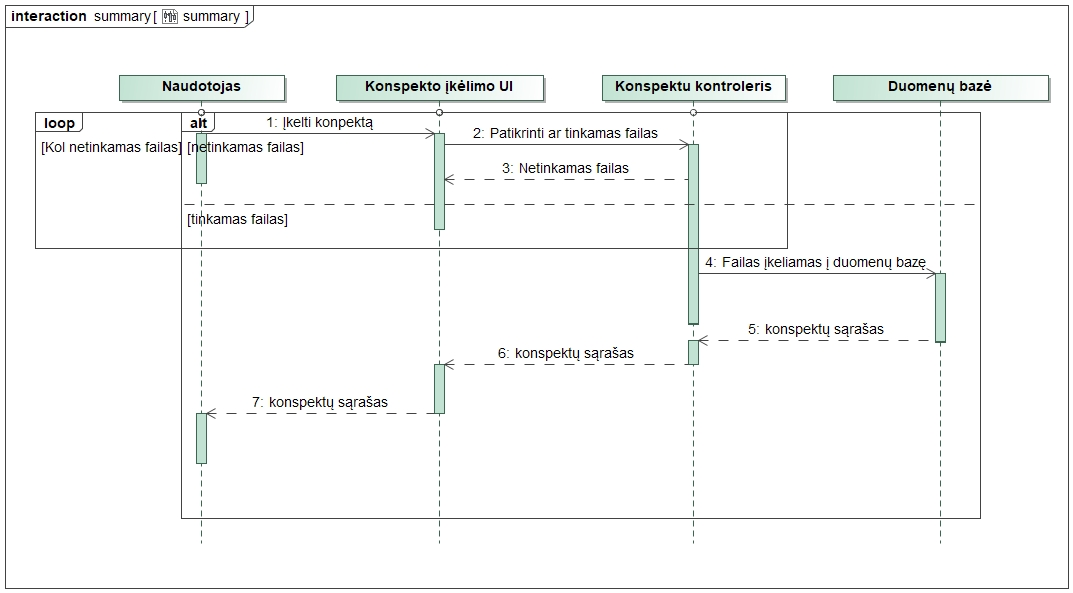
\includegraphics[width=\linewidth]{img/summary.jpg}
	\caption{Proceso „Konspekto įkėlimas“ sekų diagrama}
	\label{fig:summary}
\end{figure}
\newpage

\section{NEFUNKCINIAI REIKALAVIMAI}
2-ame skyriuje pateikiami nefunkciniai reikalavimai bei jų svarba. Aprašoma, kaip sistema turi veikti ir kaip ji turi būti kuriama.
\subsection{Vidinių interfeisų reikalavimai}
	\begin{table}[H]
	\caption{Nefunkciniai reikalavimai. Vidinių interfeisų reikalavimai.}
	\begin{tabular}{|p{1cm}|p{1cm}|p{11,5cm}|p{3,5cm}|}
	\hline 
\rowcolor{gray!50}
		\multicolumn{2}{|c|}{{\bfseries Kodas}}&
		\multicolumn{1}{c|}{{\bfseries Reikalavimas}}&
		\multicolumn{1}{c|}{{\bfseries Svarba}}\\
\hline
\rowcolor{lightgray}
\multicolumn{4}{|c|}{Vidinių interfeisų reikalavimai}\\		

\hline
\multicolumn{4}{|c|}{\bfseries OS naudojimo reikalavimai}\\	

\hline
	\multicolumn{2}{|c|}{NFR 1.1}&
	{Tinklapis pritaikytas tiek kompiuteriams, tiek mobiliesiems įrenginiams.
}&		
	\multicolumn{1}{c|}{Būtina}\\
\hline
	\multicolumn{1}{|c}{}&
	\multicolumn{1}{c|}{NFR 1.2}&
	{Puslapis pasiekiamas per visas populiariausias naršykles
(Google Chrome, Mozilla Firefox, IE (nuo 8 versijos), Edge, Safari).
}&		
	\multicolumn{1}{c|}{Būtina}\\

	\hline
\multicolumn{4}{|c|}{\bfseries Sąveikos su DB reikalavimai}\\		
				
	\hline
		\multicolumn{1}{|c}{}&
		\multicolumn{1}{c|}{NFR 2.1}&
		{Tinklapis turi turėti duomenų bazę, kurioje saugomi naudotojų duomenys, renginiai, D.U.K., konspektai bei dėstytojų puslapių informacija.
		}&
		\multicolumn{1}{c|}{Būtina}\\	
\hline		
		\multicolumn{1}{|c}{}&
		\multicolumn{1}{c|}{NFR 2.2}&
		{Duomenys saugomi reliaciniu būdu, naudojama MySQL
duomenų bazių valdymo sistema.
		}&
		\multicolumn{1}{c|}{Būtina}\\		
		
		\hline		
		\multicolumn{1}{|c}{}&
		\multicolumn{1}{c|}{NFR 2.3}&
		{Naudojama Microsoft Azure SQL Database paslauga.
		}&
		\multicolumn{1}{c|}{Pageidautina}\\	
		
		
\hline
\multicolumn{4}{|c|}{\bfseries Dokumentų mainų reikalavimai}\\		
		
	\hline
		\multicolumn{2}{|c|}{NFR 3.1}&
		{Naudotojų įkeliamos nuotraukos turi būti,.jpg, .png, .bmp formato bei neviršyti 5MB dydžio.
		}&
		\multicolumn{1}{c|}{Būtina}\\
		
	\hline
\multicolumn{4}{|c|}{\bfseries Darbo kompiuterių tinkluose reikalavimai}\\		
			
	\hline
		\multicolumn{1}{|c}{}&
		\multicolumn{1}{c|}{NFR 4.1}&
		{Duomenys perduodami naudojant HTTPS protokolą.
		}&
		\multicolumn{1}{c|}{Būtina}\\	
		
	\hline
\multicolumn{4}{|c|}{\bfseries Sąveikos su kitomis programomis reikalavimai}\\	
\hline
		\multicolumn{1}{|c}{}&
		\multicolumn{1}{c|}{NFR 5.1}&
		{Vartotojo autentifikacija vykdoma per is.vu.lt sistemą.
		}&
		\multicolumn{1}{c|}{Būtina}\\
		
	\hline
\multicolumn{4}{|c|}{\bfseries Programavimo aplinkos reikalavimai}\\	
\hline
		\multicolumn{1}{|c}{}&
		\multicolumn{1}{c|}{NFR 6.1}&
		{Tinklapis kuriamas PHP programavimo kalba, naudojant
Symfony karkasą.
		}&
		\multicolumn{1}{c|}{Būtina}\\		

\hline
		\multicolumn{1}{|c}{}&
		\multicolumn{1}{c|}{NFR 6.2}&
		{Kodo saugojimui ir dalinimuisi naudojama privati Github repositorija.
		}&
		\multicolumn{1}{c|}{Pageidautina}\\	
		
\hline
		\multicolumn{1}{|c}{}&
		\multicolumn{1}{c|}{NFR 6.3}&
		{Naudojama PHPStorm programavimo aplinka.
		}&
		\multicolumn{1}{c|}{Pageidautina}\\									

	\hline
	\end{tabular}		
	\end{table}
	
	
\subsection{Veikimo reikalavimai}
\begin{table}[H]
	\caption{Nefunkciniai reikalavimai. Veikimo reikalavimai.}
	\begin{tabular}{|p{1cm}|p{1cm}|p{11,5cm}|p{3,5cm}|}
	\hline 
\rowcolor{gray!50}
		\multicolumn{2}{|c|}{{\bfseries Kodas}}&
		\multicolumn{1}{c|}{{\bfseries Reikalavimas}}&
		\multicolumn{1}{c|}{{\bfseries Svarba}}\\
\hline
\rowcolor{lightgray}
\multicolumn{4}{|c|}{Veikimo reikalavimai}\\		

\hline
\multicolumn{4}{|c|}{\bfseries Vaizdavimo reikalavimai}\\	

\hline
	\multicolumn{2}{|c|}{NFR 7.1}&
	{Tinklapis turi būti palaikomas visose populiariausiose naršyklėse (IE (nuo 8 versijos), Edge, Chrome, Safari, Firefox).
}&		
	\multicolumn{1}{c|}{Būtina}\\
\hline
	\multicolumn{1}{|c}{}&
	\multicolumn{1}{c|}{NFR 7.2}&
	{Keičiant naršyklės dydį, tinklapis vaizdą pritaiko automatiškai.).
}&		
	\multicolumn{1}{c|}{Būtina}\\

\hline
	\multicolumn{1}{|c}{}&
	\multicolumn{1}{c|}{NFR 7.3}&
	{Data turi būti vaizduojama formatu YYYY-MM-DD, kur
YYYY – metai, MM – mėnuo, DD – diena.
}&		
	\multicolumn{1}{c|}{Būtina}\\
	
	\hline
	\multicolumn{1}{|c}{}&
	\multicolumn{1}{c|}{NFR 7.4}&
	{Laikas turi būti vaizduojamas formatu hh:mm, kur hh - valandos, mm - minutės.
}&		
	\multicolumn{1}{c|}{Būtina}\\
	
		\hline
	\multicolumn{1}{|c}{}&
	\multicolumn{1}{c|}{NFR 7.5}&
	{Pavadinimai – ne daugiau 50 simbolių.
}&		
	\multicolumn{1}{c|}{Būtina}\\

	\hline
\multicolumn{4}{|c|}{\bfseries Robastiškumo reikalavimai}\\		
				
	\hline
		\multicolumn{1}{|c}{}&
		\multicolumn{1}{c|}{NFR 8.1}&
		{Sistemoje turi būti įdiegtos apsaugos priemonės nuo duomenų sugadinimo, praradimo, klaidingų duomenų įvedimo į DB.
		}&
		\multicolumn{1}{c|}{Būtina}\\	
\hline		
		\multicolumn{1}{|c}{}&
		\multicolumn{1}{c|}{NFR 8.2}&
		{Pranešti naudotojui, jei interneto ryšys nutrūko.
		}&
		\multicolumn{1}{c|}{Pageidautina}\\		
				
\hline
\multicolumn{4}{|c|}{\bfseries Našumo reikalavimai}\\		
		
	\hline
		\multicolumn{2}{|c|}{NFR 9.1}&
		{Užklausai įvykdyti turi užtekti ne daugiau nei 5 sekundžių.
		}&
		\multicolumn{1}{c|}{Būtina}\\
		
	\hline
\multicolumn{4}{|c|}{\bfseries Darbo kompiuterių tinkluose reikalavimai}\\		
			
	\hline
		\multicolumn{1}{|c}{}&
		\multicolumn{1}{c|}{NFR 10.1}&
		{Svetainės talpinimo (hostingo) planas turi būti parinktas atsižvelgiant į prognozuojamą klientų srautą. Rekomenduojamas duomenų srautas – 50GB/mėn., vieta serveryje - iki 3GB.
		}&
		\multicolumn{1}{c|}{Būtina}\\
		
		\hline
		\multicolumn{1}{|c}{}&
		\multicolumn{1}{c|}{NFR 10.1}&
		{Didžiausia leistina tinklapio sistemos apkrova yra 1000 naudotojų, prisijungusių vienu metu.
		}&
		\multicolumn{1}{c|}{Būtina}\\
	\hline
	\end{tabular}		
	\end{table}
\subsection{Diegimo reikalavimai}
\begin{table}[H]
	\caption{Nefunkciniai reikalavimai. Diegimo reikalavimai.}
	\begin{tabular}{|p{1cm}|p{1cm}|p{11,5cm}|p{3,5cm}|}
	\hline 
\rowcolor{gray!50}
		\multicolumn{2}{|c|}{{\bfseries Kodas}}&
		\multicolumn{1}{c|}{{\bfseries Reikalavimas}}&
		\multicolumn{1}{c|}{{\bfseries Svarba}}\\
\hline
\rowcolor{lightgray}
\multicolumn{4}{|c|}{Diegimo reikalavimai}\\		

\hline
\multicolumn{4}{|c|}{\bfseries Ruošinio reikalavimai}\\	

\hline
	\multicolumn{2}{|c|}{NFR 11.1}&
	{Dokumentacija
}&		
	\multicolumn{1}{c|}{Būtina}\\
\hline
	\multicolumn{1}{|c}{}&
	\multicolumn{1}{c|}{NFR 11.2}&
	{Hostingo prisijungimo duomenys.
}&		
	\multicolumn{1}{c|}{Būtina}\\

\hline
	\multicolumn{1}{|c}{}&
	\multicolumn{1}{c|}{NFR 11.3}&
	{MS Azure prisijungimo duomenys.
}&		
	\multicolumn{1}{c|}{Pageidautina}\\
	
	
	\hline
\multicolumn{4}{|c|}{\bfseries Instaliavimo reikalavimai}\\		
				
	\hline
		\multicolumn{1}{|c}{}&
		\multicolumn{1}{c|}{NFR 12.1}&
		{Apsilankęs internetiniame pusalpyje, vartotojas privalo sutikti su slapukų naudojimo sąlygomis.
		}&
		\multicolumn{1}{c|}{Būtina}\\	
				
\hline
\multicolumn{4}{|c|}{\bfseries Pradinio DB kaupimo reikalavimai}\\		
		
	\hline
		\multicolumn{2}{|c|}{NFR 13.1}&
		{Turi būti sukurtos lentelės.}&
		\multicolumn{1}{c|}{Būtina}\\
		
	\hline
		\multicolumn{2}{|c|}{NFR 13.2}&
		{Naudotojų lentelėje turi būti administratoriaus duomenys.}&
		\multicolumn{1}{c|}{Būtina}\\	
		
	\hline
\multicolumn{4}{|c|}{\bfseries Sistemos įsisavinamumo reikalavimai}\\		
			
	\hline
		\multicolumn{1}{|c}{}&
		\multicolumn{1}{c|}{NFR 14.1}&
		{Sistema turi funkcionuoti dvejomis kalbomis: lietuvių ir anglų.}&
		\multicolumn{1}{c|}{Būtina}\\
		
		\hline
		\multicolumn{1}{|c}{}&
		\multicolumn{1}{c|}{NFR 14.2}&
		{Negali būti klaidinančių nuorodų.}&
		\multicolumn{1}{c|}{Būtina}\\
		
		\hline
		\multicolumn{1}{|c}{}&
		\multicolumn{1}{c|}{NFR 14.3}&
		{Ikonos turi atspindėti mygtuko panaudojimą.}&
		\multicolumn{1}{c|}{Būtina}\\
		
	\hline
	\end{tabular}		
	\end{table}
\subsection{Aptarnavimo ir priežiūros reikalavimai}
\begin{table}[H]
	\caption{Nefunkciniai reikalavimai. Aptarnavimo ir priežiūros reikalavimai.}
	\begin{tabular}{|p{1cm}|p{1cm}|p{11,5cm}|p{3,5cm}|}
	\hline 
\rowcolor{gray!50}
		\multicolumn{2}{|c|}{{\bfseries Kodas}}&
		\multicolumn{1}{c|}{{\bfseries Reikalavimas}}&
		\multicolumn{1}{c|}{{\bfseries Svarba}}\\
\hline
\rowcolor{lightgray}
\multicolumn{4}{|c|}{Aptarnavimo ir priežiūros reikalavimai}\\		

\hline
	\multicolumn{2}{|c|}{NFR 15.1}&
	{Atsiradęs naujas funkcionalumas turi būti įdiegtas per 5 darbo dienas.
}&		
	\multicolumn{1}{c|}{Būtina}\\
\hline
	\multicolumn{1}{|c}{}&
	\multicolumn{1}{c|}{NFR 15.2}&
	{Rasta klaida turi būti ištaisyta per 2 darbo dienas.
}&		
	\multicolumn{1}{c|}{Būtina}\\

\hline
	\multicolumn{1}{|c}{}&
	\multicolumn{1}{c|}{NFR 15.3}&
	{Į naudotojo laiškus su pastebėjimais ir skundais atsakyti reikia per 3 darbo dienas.
}&		
	\multicolumn{1}{c|}{Pageidautina}\\
	
\hline
	\multicolumn{1}{|c}{}&
	\multicolumn{1}{c|}{NFR 15.4}&
	{Jei dėl planuojamo atnaujinimo reikės trumpam sustabdyti
sistemos veiklą, naudotojai turi būti iš anksto įspėti ne mažiau nei prieš 24 val.
}&		
	\multicolumn{1}{c|}{Pageidautina}\\	
			
	\hline
	\end{tabular}		
	\end{table}
\subsection{Tiražuojamumo reikalavimai}
\begin{table}[H]
	\caption{Nefunkciniai reikalavimai. Tiražuojamumo reikalavimai.}
	\begin{tabular}{|p{1cm}|p{1cm}|p{12,5cm}|p{3,5cm}|}
	\hline 
\rowcolor{gray!50}
		\multicolumn{2}{|c|}{{\bfseries Kodas}}&
		\multicolumn{1}{c|}{{\bfseries Reikalavimas}}&
		\multicolumn{1}{c|}{{\bfseries Svarba}}\\
\hline
\rowcolor{lightgray}
\multicolumn{4}{|c|}{Tiražuojamumo reikalavimai}\\		

\hline
	\multicolumn{2}{|c|}{NFR 16.1}&
	{Internetinė svetainė turi veikti bet kuriame įrenginyje, kuris turi naršyklę ir interneto ryšį.
}&		
	\multicolumn{1}{c|}{Būtina}\\
			
	\hline
	\end{tabular}		
	\end{table}
\subsection{Apsaugos reikalavimai}
\begin{table}[H]
	\caption{Nefunkciniai reikalavimai. Apsaugos reikalavimai.}
	\begin{tabular}{|p{1cm}|p{1cm}|p{12,5cm}|p{3,5cm}|}
	\hline 
\rowcolor{gray!50}
		\multicolumn{2}{|c|}{{\bfseries Kodas}}&
		\multicolumn{1}{c|}{{\bfseries Reikalavimas}}&
		\multicolumn{1}{c|}{{\bfseries Svarba}}\\
\hline
\rowcolor{lightgray}
\multicolumn{4}{|c|}{Apsaugos reikalavimai}\\		

\hline
	\multicolumn{2}{|c|}{NFR 17.1}&
	{Naudotojui prisijungiant prie sistemos vykdoma jo identifikacija.
}&		
	\multicolumn{1}{c|}{Būtina}\\
	
\hline
	\multicolumn{2}{|c|}{NFR 17.2}&
	{Atsarginės DB kopijos daromos ne rečiau nei kas savaitę.
}&		
	\multicolumn{1}{c|}{Būtina}\\	
	
\hline
	\multicolumn{2}{|c|}{NFR 17.3}&
	{Jei naudotojas neaktyvus ilgiau nei 30 minučių, jis turi būti automatiškai atjungiamas nuo sistemos.
}&		
	\multicolumn{1}{c|}{Būtina}\\		
			
	\hline
	\end{tabular}		
	\end{table}
\subsection{Juridiniai reikalavimai}
\begin{table}[H]
	\caption{Nefunkciniai reikalavimai. Juridiniai reikalavimai.}
	\begin{tabular}{|p{1cm}|p{1cm}|p{12,5cm}|p{3,5cm}|}
	\hline 
\rowcolor{gray!50}
		\multicolumn{2}{|c|}{{\bfseries Kodas}}&
		\multicolumn{1}{c|}{{\bfseries Reikalavimas}}&
		\multicolumn{1}{c|}{{\bfseries Svarba}}\\
\hline
\rowcolor{lightgray}
\multicolumn{4}{|c|}{Juridiniai reikalavimai}\\		

\hline
	\multicolumn{2}{|c|}{NFR 18.1}&
	{Kuriant sistemą projekto komanda neturi naudotis nelegalia
programine įranga.
}&		
	\multicolumn{1}{c|}{Būtina}\\
	
\hline
	\multicolumn{2}{|c|}{NFR 18.2}&
	{Internetinėje svetainėje turi būti galimybė peržiūrėti naudojimosi sąlygas.
}&		
	\multicolumn{1}{c|}{Būtina}\\				
	\hline
	\end{tabular}		
	\end{table}
\newpage

\section{VARTOTOJO SĄSAJOS REIKALAVIMAI}
3 skyriuje pateikiami vartotojo sąsajos reikalavimai, kuriuose pateikiama informaciją apie sistemos grafinį vaizdą, kurį mato vartotojas. Nagrinėjami naudotojui matomi puslapiai, ikonos, simboliai bei mygtukai, pavaizduoti prototipuose (žr. 1 priedas). Taip pat aprašomos jų funkcijos, paskirtys bei svarbumas.

\subsection{Dalykinės srities metaforos reikalavimai}
\begin{table}[H]
	\caption{Vartotojo interfeiso reikalavimai. Dalykinės srities metaforos reikalavimai.}
	\begin{tabular}{|p{1cm}|p{1cm}|p{12,5cm}|p{3,5cm}|}
	\hline
\rowcolor{lightgray}
\multicolumn{4}{|c|}{1. Dalykinės srities metaforos reikalavimai}\\		
	\hline 
\rowcolor{gray!50}
		\multicolumn{2}{|c|}{{\bfseries Kodas}}&
		\multicolumn{1}{c|}{{\bfseries Reikalavimas}}&
		\multicolumn{1}{c|}{{\bfseries Svarba}}\\
\hline
	\multicolumn{2}{|c|}{VIR 1.1}&
	{Pagrindinio puslapio atidarymas arba perkrovimas yra vaizduojamas puslapio logotipu}&		
	\multicolumn{1}{c|}{Būtinas}\\
\hline
	\multicolumn{2}{|c|}{VIR 1.2}&
	{Renginio arba naujienos įkėlimas yra vaizduojamas pliuso simboliu.}&		
	\multicolumn{1}{c|}{Pageidautina}\\	
\hline
	\multicolumn{2}{|c|}{VIR 1.3}&
	{Renginio arba naujienos redagavimas yra vaizduojamas pieštuko simboliu.}&		
	\multicolumn{1}{c|}{Pageidautina}\\	
\hline
	\multicolumn{2}{|c|}{VIR 1.4}&
	{Renginiai išdėstyti nuo eilės tvarka nuo artimiausios datos iki tolimiausios}&		
	\multicolumn{1}{c|}{Būtina}\\				
	\hline
\end{tabular}		
\end{table}


\begin{longtable}{|p{2cm}|p{11,5cm}|p{2cm}|}\toprule
\caption{Vartotojo interfeiso reikalavimai. Užduočių reikalavimai}\\
\hline  \rowcolor{lightgray} 
\multicolumn{3}{|c|}{2. Užduočių reikalavimai}\\ \hline 
\multicolumn{1}{|l|}{\textbf{Kodas}} & \multicolumn{1}{c|}{\textbf{Reikalavimas}} & \multicolumn{1}{c|}{\textbf{Svarba}} \\ \hline 
\multicolumn{3}{|c|}{Neprisiregistravusio naudotojo sąsajos užduotys}\\ \hline
{VIR3.1}&{Prisiregistruoti prie aplikacijos}&{Būtinas} \\ \hline
{VIR2.2}&{Susipažinti su puslapio taisyklėmis}&{Būtinas}\\ \hline
\multicolumn{3}{|c|}{Dėstytojo sąsajos užduotys}\\ \hline
{VIR3.1}&{Prisijungti prie savo paskyros}&{Būtinas}\\ \hline
{VIR3.2}&{Redaguoti savo prisijungimo slaptažodį}&{Būtinas}\\ \hline
{VIR3.3}&{Atsijungti iš savo paskyros}&{Būtinas}\\ \hline
{VIR3.4}&{Pridėti naujieną}&{Būtinas}\\ 	\hline
{VIR3.5}&{Redaguoti renginį}&{Būtinas}\\	\hline
{VIR3.6}&{Ištrinti renginį}&{Būtinas}\\ 	\hline
{VIR3.7}&{Pridėti renginį}&{Būtinas}\\ 	\hline
{VIR3.8}&{Redaguoti renginį}&{Būtinas}\\ 	\hline
{VIR3.9}&{Ištrinti renginį}&{Būtinas}\\	\hline
{VIR3.10}&{Siųsti žinutę}&{Būtinas}\\ 	\hline
{VIR3.11}&{Peržiūrėti visas žinutes}&{Būtinas}\\ 	\hline
{VIR3.12}&{Gauti žinutes}&{Būtinas}\\ 	\hline
{VIR3.13}&{Peržvelgti visas naujienas}&{Būtinas}\\	\hline
{VIR3.14}&{Peržvelgti visus renginius}&{Būtinas}\\	\hline
{VIR3.15}&{Peržiūrėti D.U.K.}&{Būtinas}\\	\hline
{VIR3.16}&{Pridėti D.U.K.}&{Būtinas}\\ 	\hline
{VIR3.17}&{Peržiūrėti D.U.K.}&{Būtinas}\\	\hline
{VIR3.18}&{Peržvelgti visus dėstytojus}&{Būtinas}\\ 	\hline
{VIR3.19}&{Redaguoti asmeninį tinklalapį}&{Būtinas}\\ 	\hline
\multicolumn{3}{|c|}{Studento sąsajos užduotys}\\	\hline
{VIR4.1}&{Prisijungti prie savo paskyros}&{Būtinas}\\	\hline
{VIR4.2}&{Redaguoti savo prisijungimo slaptažodį}&{Būtinas}\\	\hline
{VIR4.3}&{Atsijungti iš savo paskyros}&{Būtinas}\\	\hline
{VIR4.4}&{Siųsti žinutę}&{Būtinas}\\	\hline
{VIR4.5}&{Peržiūrėti visas žinutes}&{Būtinas}\\	\hline
{VIR4.6}&{Gauti žinutes}&{Būtinas}\\	\hline
{VIR4.7}&{Peržvelgti visas naujienas}&{Būtinas}\\	\hline
{VIR4.8}&{Peržvelgti visus renginius}&{Būtinas}\\	\hline
{VIR4.9}&{Peržiūrėti D.U.K.}&{Būtinas}\\	\hline
{VIR4.10}&{Peržiūrėti D.U.K.}&{Būtinas}\\	\hline
{VIR4.11}&{Peržvelgti visus dėstytojus}&{Būtinas}\\	\hline
{VIR4.12}&{Peržiūrėti konkretaus dėstytojo puslapį ir informaciją jame}&{Būtinas}\\	\hline
{VIR4.13}&{Peržiūrėti visus konspektus}&{Būtinas}\\	\hline
{VIR4.14}&{Įkelti konspektą}&{Būtinas}\\	\hline
\multicolumn{3}{|c|}{Administratoriaus sąsajos reikalavimai}\\	\hline
{VIR5.1}&{Pridėti naujienas/renginius/D.U.K.}&{Būtinas}\\	\hline
{VIR5.2}&{Peržiūrėti naujienas/renginius/D.U.K. ir pašalinti nebeaktualius}&{Būtinas}\\	\hline
{VIR5.3}&{Kurti sąrašus duomenų bazėje}&{Būtinas}\\	\hline
{VIR5.4}&{Atnaujinti tinklalapį}&{Būtinas}\\	\hline
{VIR5.5}&{Patikrinti konspektų turinį}&{Būtinas}\\	\hline
{VIR5.6}&{Taisyti tinklalapio klaidas}&{Būtinas}\\	\hline
{VIR5.7}&{Blokuoti naudotojus}&{Būtinas}\\	\hline
\multicolumn{3}{|c|}{Bendri reikalavimai}\\	\hline
{VIR6.1}&{Puslapio viršuje visada esantis meniu}&{Būtinas}\\	\hline
{VIR6.2}&{Teksto įvedimo formų laukai}&{Būtinas}\\	\hline
{VIR6.3}&{Ikonos}&{Būtinas}\\	\hline
{VIR6.4}&{Matomas atsijungimo mygtukas}&{Būtinas}\\	\hline
\end{longtable}

\subsection{Užduočių formulavimo kalbos reikalavimai}
\begin{table}[H]
	\caption{Vartotojo interfeiso reikalavimai. Užduočių formulavimo kalbos reikalavimai}
\begin{tabular}{|p{1cm}|p{1cm}|p{11,5cm}|p{3,5cm}|}
	\hline
\rowcolor{lightgray}
\multicolumn{4}{|c|}{3. Užduočių formulavimo kalbos reikalavimai}\\		
	\hline 
\rowcolor{gray!50}
\multicolumn{2}{|c|}{{\bfseries Kodas}}&\multicolumn{1}{c|}{{\bfseries Reikalavimas}}&\multicolumn{1}{c|}{{\bfseries Svarba}}\\
\hline
\multicolumn{4}{|c|}{Įrankiai skirti naudotojui naudotis aplikacija}\\	\hline
\multicolumn{2}{|c|}{VIR7.1}&{Grafinis meniu – vartotojo sąsaja su tinklalapiu}&\multicolumn{1}{c|}{Būtinas}\\
\hline
\multicolumn{2}{|c|}{VIR7.2}&{Mygtukai – naudojami siekiant patekti į kitus tinklalapio langus}&\multicolumn{1}{c|}{Būtinas}\\
\hline
\multicolumn{2}{|c|}{VIR7.3}&{Ikonos – interfeise naudojamos piktogramos}&\multicolumn{1}{c|}{Būtinas}\\
\hline
\multicolumn{2}{|c|}{VIR7.4}&{Patvirtinimo langai - langai prašantys naudotojo dar kartą patvirtinti tam tikrą svarbų veiksmą}&\multicolumn{1}{c|}{Būtinas}\\
\hline
\multicolumn{2}{|c|}{VIR7.5}&{Įvedimo laukai – naudojami naudotojui įvesti tekstinius duomenis}&\multicolumn{1}{c|}{Būtinas}\\
\hline
\multicolumn{2}{|c|}{VIR8.1}&{Naudotojo prisijungimo vardas turi būti validus el. pašto adresas egzistuojantis VU sistemoje}&\multicolumn{1}{c|}{Būtinas}\\
\hline
\multicolumn{2}{|c|}{VIR9.1}&{Naudotojo slaptažodis turi būti sudarytas iš raidžių (didžiųjų ir mažųjų), skaitmenų ir specialių simbolių}&\multicolumn{1}{c|}{Būtinas}\\
\hline
\multicolumn{2}{|c|}{VIR9.2}&{Slaptažodis turi būti ne trumpesnis nei 8 simboliai}&\multicolumn{1}{c|}{Būtinas}\\
\hline
\end{tabular}		
\end{table}

 \subsection{Užduočių formulavimo protokolo reikalavimai}
 
 \begin{longtable}{|p{2cm}|p{12,5cm}|p{1,5cm}|}\toprule
 \caption{Vartotojo interfeiso reikalavimai. Užduočių formulavimo protokolo reikalavimai}\\
    \hline  \rowcolor{lightgray} \multicolumn{3}{|c|}{4. Užduočių formulavimo protokolo reikalavimai}\\	\hline
    \multicolumn{1}{|c|}{\bf Kodas} & \multicolumn{1}{c|}{\bf Reikalavimas} & \multicolumn{1}{c|}{\bf Svarba} \\ \hline
    \multicolumn{3}{|c|}{Prisiregistravimas prie tinklalapio}\\ \hline
   {VIR10.1}&{Norėdamas prisiregistruoti naudotojas turi paspausti mygtuką „Registruotis“. Paspaudus jį išmetamas registracijos langas, kuriame naudotojas suveda savo duomenis (el. paštas, vardas, pavardė, slaptažodis, pasirenkama dėstytojo/studento kategorija, pasirinkus dėstytoją suvedamas dėstytojo identifikacijos kodas)}&{Būtinas}\\  \hline
{VIR10.2}&{Paspaudus mygtuką „Registruotis“ registracijos lange tikrinama ar duomenys suvesti teisingai ir ar tokio naudotojo dar nėra duomenų bazėje, jei viskas gerai, naudotojas prijungiamas prie paskyros. Kitu atveju į ekraną išmetamos žinutės prie tų laukų, kurie yra suvesti klaidingai}&{Būtinas}\\ \hline
\multicolumn{3}{|c|}{Prisijungimas prie tinklalapio}\\ \hline
{VIR11.1}&{Prisijungti gali tik registruotas naudotojas. Tai padaryti gali paspaudęs mygtuką „Prisijungti“ ir išmestame lange suvedęs savo prisijungimo duomenis (el.paštą, slaptažodį)}&{Būtinas}\\ \hline
{VIR11.2}&{Paspaudus tvirtinantį prisijungimą mygtuką „Prisijungti“ duomenys yra patikrinami duomenų bazėje ir, jei viskas teisinga, naudotojas yra prijungiamas. Jei prisijungimas klaidingas, naudotojui išmetama žinutė, kad prijungimas nepavyko, prašoma patikrinti suvestus laukus}&{Būtinas}\\ \hline
{VIR11.3}&{Prisijungiant galima pažymėti varnelę prie „Prisiminti mane“ ir kitą kartą naudotojas bus prijungiamas automatiškai, nevedant duomenų iš naujo}&{Būtinas}\\ \hline
\multicolumn{3}{|c|}{Pamirštas slaptažodis}\\ \hline
{VIR12.1}&{Pamiršus slaptažodį galima paspausti ant mygtuko „Pamiršau slaptažodį“. Atsiradusiame lange reikia įvesti el.paštą, kuriuo naudotojas prisijungia.}&{Būtinas}\\ \hline
{VIR12.2}&{Sistema radusi tokį el.paštą duomenų bazėje išsiunčia nuorodą nurodytu el.pašto adresu nukreipiančiu į formą leidžiančią pasikeisti slaptažodį}&{Būtinas}\\ \hline
 \multicolumn{3}{|c|}{Pagrindinis juostinis meniu}\\ \hline
{VIR13.1}&{Vaizduojamas viršutinėje puslapio dalyje, matomas kiekviename pasirinkimų lange}&{Būtinas}\\ \hline
{VIR13.2}&{Kairiame kampe vaizduojamas tinklalapio logotipas ir pavadinimas „SocialVU“}&{Būtinas}\\ \hline
{VIR13.3}&{Dešiniame kampe rodomas naudotojo el.paštas, kuris nukreipia į asmeninį profilį, kuriame galima rasti prisijungimo informaciją, ir atsijungimo mygtukas „Atsijungti“ bei „Žinutės“}&{Būtinas}\\ \hline
{VIR13.4}&{Prisijungus dėstytojo aplinkoje šone atsiranda mygtukas „Mano puslapis“, kuris nukreipia į asmeninį dėstytojo puslapį}&{Būtinas}\\ \hline
{VIR13.5}&{„Pagrindinis“ - atverčiamas pagrindinis, naujienų, puslapis}&{Būtinas}\\ \hline
{VIR13.6}&{„D.U.K.“ - atverčiami dažniausiai užduodami klausimai su atsakymais}&{Būtinas}\\ \hline
{VIR13.7}&{„Dėstytojai“ - atverčiamas visų dėstytojų sąrašas}&{Būtinas}\\ \hline
{VIR13.8}&{„Renginiai“ - atverčiamas visų renginių sąrašas}&{Būtinas}\\ \hline
\multicolumn{3}{|c|}{„SocialVU“ logotipas}\\ \hline
{VIR14.1}&{„Renginiai“ - atverčiamas visų renginių sąrašas}&{Būtinas}\\ \hline
\multicolumn{3}{|c|}{„Renginiai“}\\ \hline
{VIR15.1}&{Pateikiamas pilnas renginių sąrašas su pavadinimu, data, trumpa informacija, kaina}&{Būtinas}\\ \hline
{VIR15.2}&{Paspaudus ant padidinamo stiklo aktyvuojamas įvesties langas, kuriame galima ieškoti renginio suvedant tai, ko ieškoma}&{Būtinas}\\ \hline
{VIR15.3}&{Paspaudus ant tekstinio lauko, kuriame galima pasirinkti datą, renginiai filtruojami pagal pasirinktą dieną}&{Būtinas}\\ \hline
{VIR15.4}&{Paspaudus ant konkretaus renginio, išmetama papildoma informacija apie jį}&{Būtinas}\\ \hline
{VIR15.5}&{Paspaudus „+“ (matoma tik dėstytojui) išmetama renginio pridėjimo forma}&{Būtinas}\\ \hline
\multicolumn{3}{|c|}{„Dėtytojai“}\\ \hline
{VIR16.1}&{Pateikiamas pilnas dėstytojų sąrašas (vardas, pavardė, dėstomų dalykų sąrašas, nuotrauka)}&{Būtinas}\\ \hline
{VIR16.2}&{Paspaudus ant padidinamo stiklo aktyvuojamas įvesties langas, kuriame galima ieškoti dėstytojo suvedant tai, ko ieškoma}&{Būtinas}\\ \hline
{VIR16.3}&{Paspaudus ant konkretaus dėstytojo, naudotojas nukreipiamas į dėstytojo puslapį}&{Būtinas}\\ \hline
\multicolumn{3}{|c|}{„D.U.K.“}\\ \hline
{VIR17.1}&{Pateikiamas pilnas D.U.K. sąrašas su atsakymais}&{Būtinas}\\ \hline
{VIR17.2}&{Paspaudus ant padidinamo stiklo aktyvuojamas įvesties langas, kuriame galima ieškoti klausimo suvedant tai, ko ieškoma}&{Būtinas}\\ \hline
{VIR17.3}&\multicolumn{1}{c|}{Paspaudus „+“ (matoma tik dėstytojui) išmetama renginio pridėjimo forma}&{Būtinas}\\ \hline
\multicolumn{3}{|c|}{„Žinutės“}\\ \hline
{VIR18.1}&{Pateikiamas pilnas naudotojo gautų žinučių sąrašas}&{Būtinas}\\ \hline
{VIR18.2}&{Paspaudus „Išsiųstos“ pateikiamas pilnas naudotojo išsiųstų žinučių sąrašas}&{Būtinas}\\ \hline
{VIR18.3}&{Paspaudus „Visos“ pateikiamas pilnas naudotojo ir gautų, ir išsiųstų žinučių sąrašas}&{Būtinas}\\ \hline
{VIR18.4}&{Paspaudus „Sukurti“ išmetama naujos žinutės forma, kurioje pasirenkamas gavėjas, bei užpildomi žinutės duomenys}&{Būtinas}\\ \hline
{VIR19.4}&{Paspaudus ant padidinamo stiklo aktyvuojamas įvesties langas, kuriame galima ieškoti žinutės suvedant tai, ko ieškoma}&{Būtinas}\\ \hline
\multicolumn{3}{|c|}{„Konspektai“ (pasiekiami tik studentui)}\\ \hline
{VIR19.1}&{Pateikiamas pilnas dėstomų dalykų sąrašas}&{Būtinas}\\ \hline
{VIR19.2}&{Pasirinkus konkretų dalyką atidaromas sukeltų konspektų sąrašas, su trumpa informacija (autoriaus vardas, pavardė, sukūrimo data)}&{Būtinas}\\ \hline
{VIR19.3}&{Pasirinkus konkretų konspektą atidaromas failo turinys}&{Būtinas}\\ \hline
{VIR19.4}&{Paspaudus ant padidinamo stiklo aktyvuojamas įvesties langas, kuriame galima ieškoti konspekto suvedant tai, ko ieškoma}&{Būtinas}\\ \hline
{VIR19.5}&{Paspaudus „+“ išmetama konspekto pridėjimo forma}&{Būtinas}\\ \hline
\multicolumn{3}{|c|}{„Mano puslapis“ (pasiekiamas tik dėstytojui)}\\ \hline
{VIR20.1}&{Pateikiamas naudotojo asmeninis puslapis, kuriame informaciją gali pateikti pats}&{Būtinas}\\ \hline
\multicolumn{3}{|c|}{„Šoninė juosta“}\\ \hline
{VIR21.1}&{Matoma dešinėje sistemos pusėje, matoma kiekviename pasirinkimų lange}&{Būtinas}\\ \hline
\multicolumn{3}{|c|}{„El. paštas“}\\ \hline
{VIR22.1}&{Paspaudus išmetama informacija apie naudotoją}&{Būtinas}\\ \hline
{VIR22.2}&{Paspaudus ant mygtuko „Pakeisti slaptažodį“ naudotojui išmetama forma, kurioje galima pasikeisti savo prisijungimo slaptažodį}&{Būtinas}\\ \hline
\end{longtable}

\subsection{Pranešimo formulavimo reikalavimai}
\begin{table}[H]
	\caption{Vartotojo interfeiso reikalavimai. Pranešimo formulavimo reikalavimai}
	\begin{tabular}{|p{2cm}|p{11,5cm}|p{2cm}|}
	\hline \rowcolor{lightgray} \multicolumn{3}{|c|}{5. Pranešimo formulavimo reikalavimai}\\	\hline 
\rowcolor{gray!50} \multicolumn{1}{|c|}{{\bfseries Kodas}}&\multicolumn{1}{c|}{{\bfseries Reikalavimas}}&\multicolumn{1}{c|}{{\bfseries Svarba}}\\ \hline
{VIR23}&	{Pranešimai turi būti parašyti laikantis gramatikos ir skyrybos taisyklių}&{Būtinas}\\ \hline	
{VIR24}&	{Pranešimai turi būti aiškūs, suprantami, kuo trumpesni bei vienareikšmiški. Aprašo tik tą sritį, dėl kurios yra išmetami naudotojui}&{Būtinas}\\ \hline	
{VIR25}&	{Patvirtinimai turi būti aiškūs, suprantami bei vienareikšmiški. Klausia tik patvirtinimo reikalingo užduočiai patvirtinti arba nutraukti}&{Būtinas}\\ \hline
\end{tabular}		
\end{table}

\subsection{Interfeiso darnos ir standartizavimo reikalavimai}
\begin{table}[H]
	\caption{Vartotojo interfeiso reikalavimai. Interfeiso darnos ir standartizavimo reikalavimai}
	\begin{tabular}{|p{2cm}|p{11,5cm}|p{2cm}|}
	\hline \rowcolor{lightgray} \multicolumn{3}{|c|}{6. Interfeiso darnos ir standartizavimo reikalavimai}\\	\hline 
\rowcolor{gray!50} \multicolumn{1}{|c|}{{\bfseries Kodas}}&\multicolumn{1}{c|}{{\bfseries Reikalavimas}}&\multicolumn{1}{c|}{{\bfseries Svarba}}\\ \hline
{VIR26}&	{Visi grafiniai objektai turi derėti tarpusavyje. Visi mygtukai, lentelės pranešimai, ikonos derančios išvaizdos.}&{Būtinas}\\ \hline	
{VIR27}&	{Tinklalapyje naudojamos vienos paletės spalvos ir lengvai įskaitomas šriftas}&{Būtinas}\\ \hline	
\end{tabular}		
\end{table}

\subsection{Interfeiso individualizavimo reikalavimai}
\begin{table}[H]
	\caption{Vartotojo interfeiso reikalavimai. Interfeiso individualizavimo reikalavimai}
	\begin{tabular}{|p{2cm}|p{11cm}|p{3cm}|}
	\hline \rowcolor{lightgray} \multicolumn{3}{|c|}{7. Interfeiso individualizavimo reikalavimai}\\	\hline 
\rowcolor{gray!50} \multicolumn{1}{|c|}{{\bfseries Kodas}}&\multicolumn{1}{c|}{{\bfseries Reikalavimas}}&\multicolumn{1}{c|}{{\bfseries Svarba}}\\ \hline
{VIR28}&	{Sistemos spalvų pasirinkimas}&{Pageidautinas}\\ \hline	
{VIR29}&	{Kalbos pasirinkimas sistemoje}&{Pageidautinas}\\ \hline	
\end{tabular}		
\end{table} 
 
\newpage

\sectionnonum{REZULTATAI}
Atliktos šios užduotys:
\\1. Pateikti aiškiai sunumeruoti ir apibrėžti kuriamo socialinio tinklapio funkciniai reikalavimai, o jų tarpusavio sąveika atvaizduota sekų diagramomis. 
\\2. Suformuluoti nefunkciniai reikalavimai. Reikalavimai išskirti į šias skiltis: vidinių interfeisų, veikimo, diegimo, aptarnavimo ir priežiūros, tiražuojamumo, apsaugos bei juridiniai.
\\3. Vartotojo sąsajos reikalavimai apibrėžti metaforos reikalavimų lentele bei suformuluotomis užduotimis įvairiems scenarijams, taip pat pateikiami darnos ir standartizavimo bei pranešimų formulavimo reikalavimai.
\\4. Atsižvelgiant į projekto pakitimus, atitinkai pataisytas pirmasis darbas (pridėtas Konspektų puslapis, papildyta užduočių diagrama, atitinkamai užduotys).

\newpage
\end{document}